\documentclass{article}
\usepackage{graphicx}
\usepackage{amsmath}
\usepackage{cite}
\usepackage{color}
\usepackage{enumitem}
\usepackage{hyperref}
\usepackage{natbib}
\usepackage{tabularx}
\usepackage{natbib}
\usepackage{ragged2e}

\title{\textbf{La digitalizzazione nelle PA}}
\author{\texttt{Alessandro Meloni GEPID}}
\date{\textit{Anno accademico 2023/2024}}

\begin{document}
\maketitle
    
\includegraphics[width = 0.9\linewidth]{Img.jpg}
\centering \tableofcontents
\newpage\centering
\section{Introduzione}
\flushleft \begin{justify}

Come potremo aver sentito e visto, nell'ultimo anno sta impennando l'utilizzo dell'Intelligenza Artificiale e varie tecnologie di machine learning in ambiti disparati; l'Italia risulta essere un po' indietro rispetto ad altre potenze europee: come ci spiegano questi grafici.
Di fatto lo sviluppo delle tecnologie odierne, sappiamo tutti, sta aprendo un forte dibattito, pertanto, risulta opportuno avere una corretta regolamentazione, sia a livello statale che sovrastatale.
In Italia ci sono varie aurorità che si occupano del settore della digitalizzazione, ognuno con particolari compiti. Noi però non andremo ad analizzarli tutti, però, per poter inquadrare il nostro discorso, è opportuno comprendere il funzionamento di un ente in particolare: l'ANAC.
L'ANAC è un ente alla quale mi sono avvicinato durante il periodo di studio in triennale, tramite un tirocinio svoltosi presso l'Ufficio Anticorruzione del Comune di Cagliari. È un ente molto complesso e che richiede un grosso impegno nel poterlo comprendere, e che sicuramente è uno dei settori che potrebbe essere maggiormente colpito (sia in positivo che in negativo, dipende dalla propria opinione) dall'avvento di tecnologie quali Blockchain, Ai e via discorrendo. Nello specifico ci soffermeremo sugli articoli che sanciscono i principi digitali del nuovo codice dei contratti pubblici (d.lgs 36/2023), e specificatamente nell'art 30, in materia di utilizzo di meccanismi automatizzati nel ciclo di vita dei contratti pubblici. Con questo paper si cerca di porre un'analisi oggettiva su quali potrebbero essere le ripercussioni, a livello organizzativo, nel mondo del lavoro e anche nel rispetto dei principi amministrativi dedotti dall'art 97 della Costituzione, senza dimenticarsi delle varie leggi specifiche in materia.
Trasversalmente verranno anche spiegate le funzioni dell'ANAC e la regolamentazione delle Autorità Amministrative Indipendenti, ma senza allontarsi troppo dal topic centrale, così da dare una visione di insieme più corretta e comprensibile.
\end{justify}

\newpage\centering
\section{Nuovo codice degli appalti}
\begin{center}
    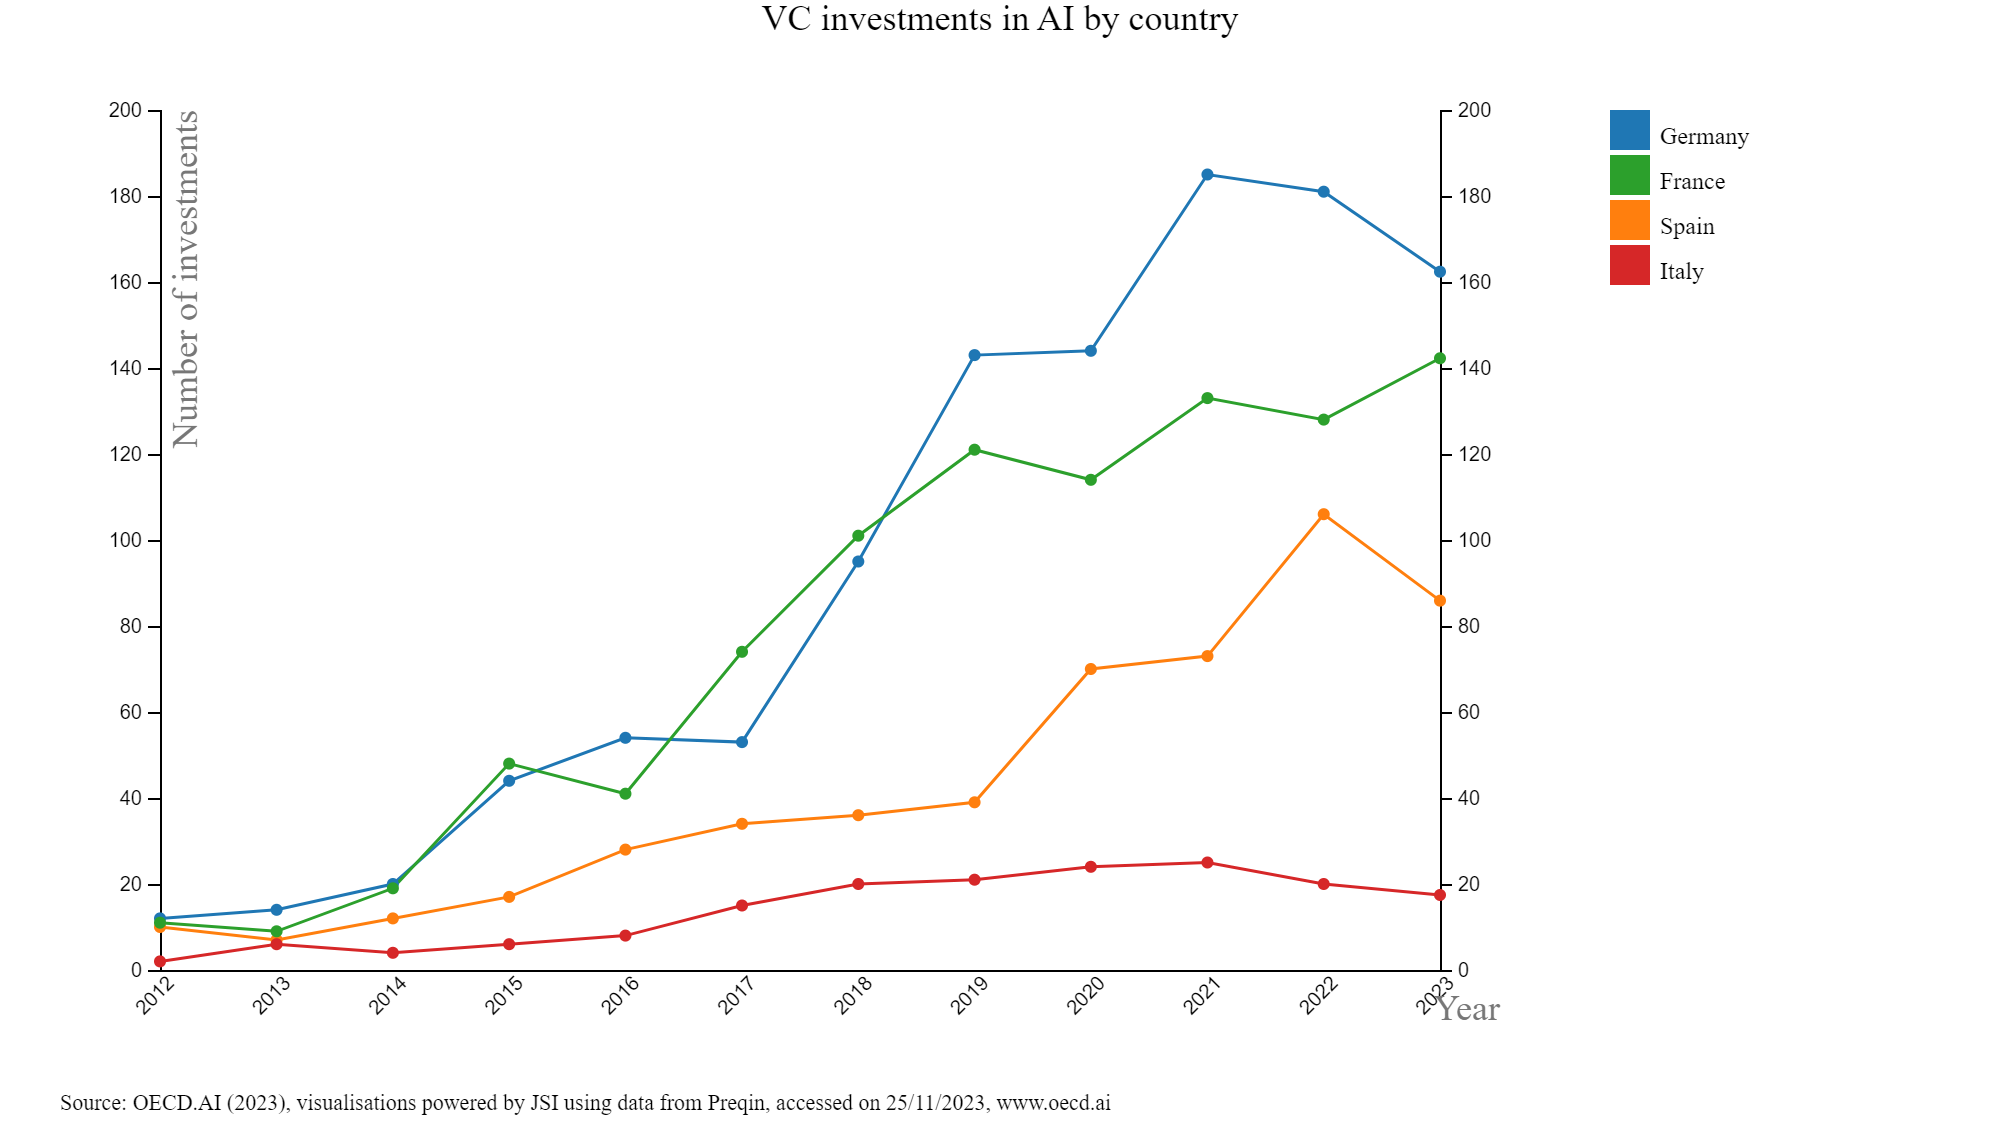
\includegraphics[width=0.3\linewidth]{Numero investimenti.png}
\end{center}
Questo grafico rappresenta il numero degli investimenti effettuati per Stato nel settore AI e Data.\label{F:numero}
\begin{center}
    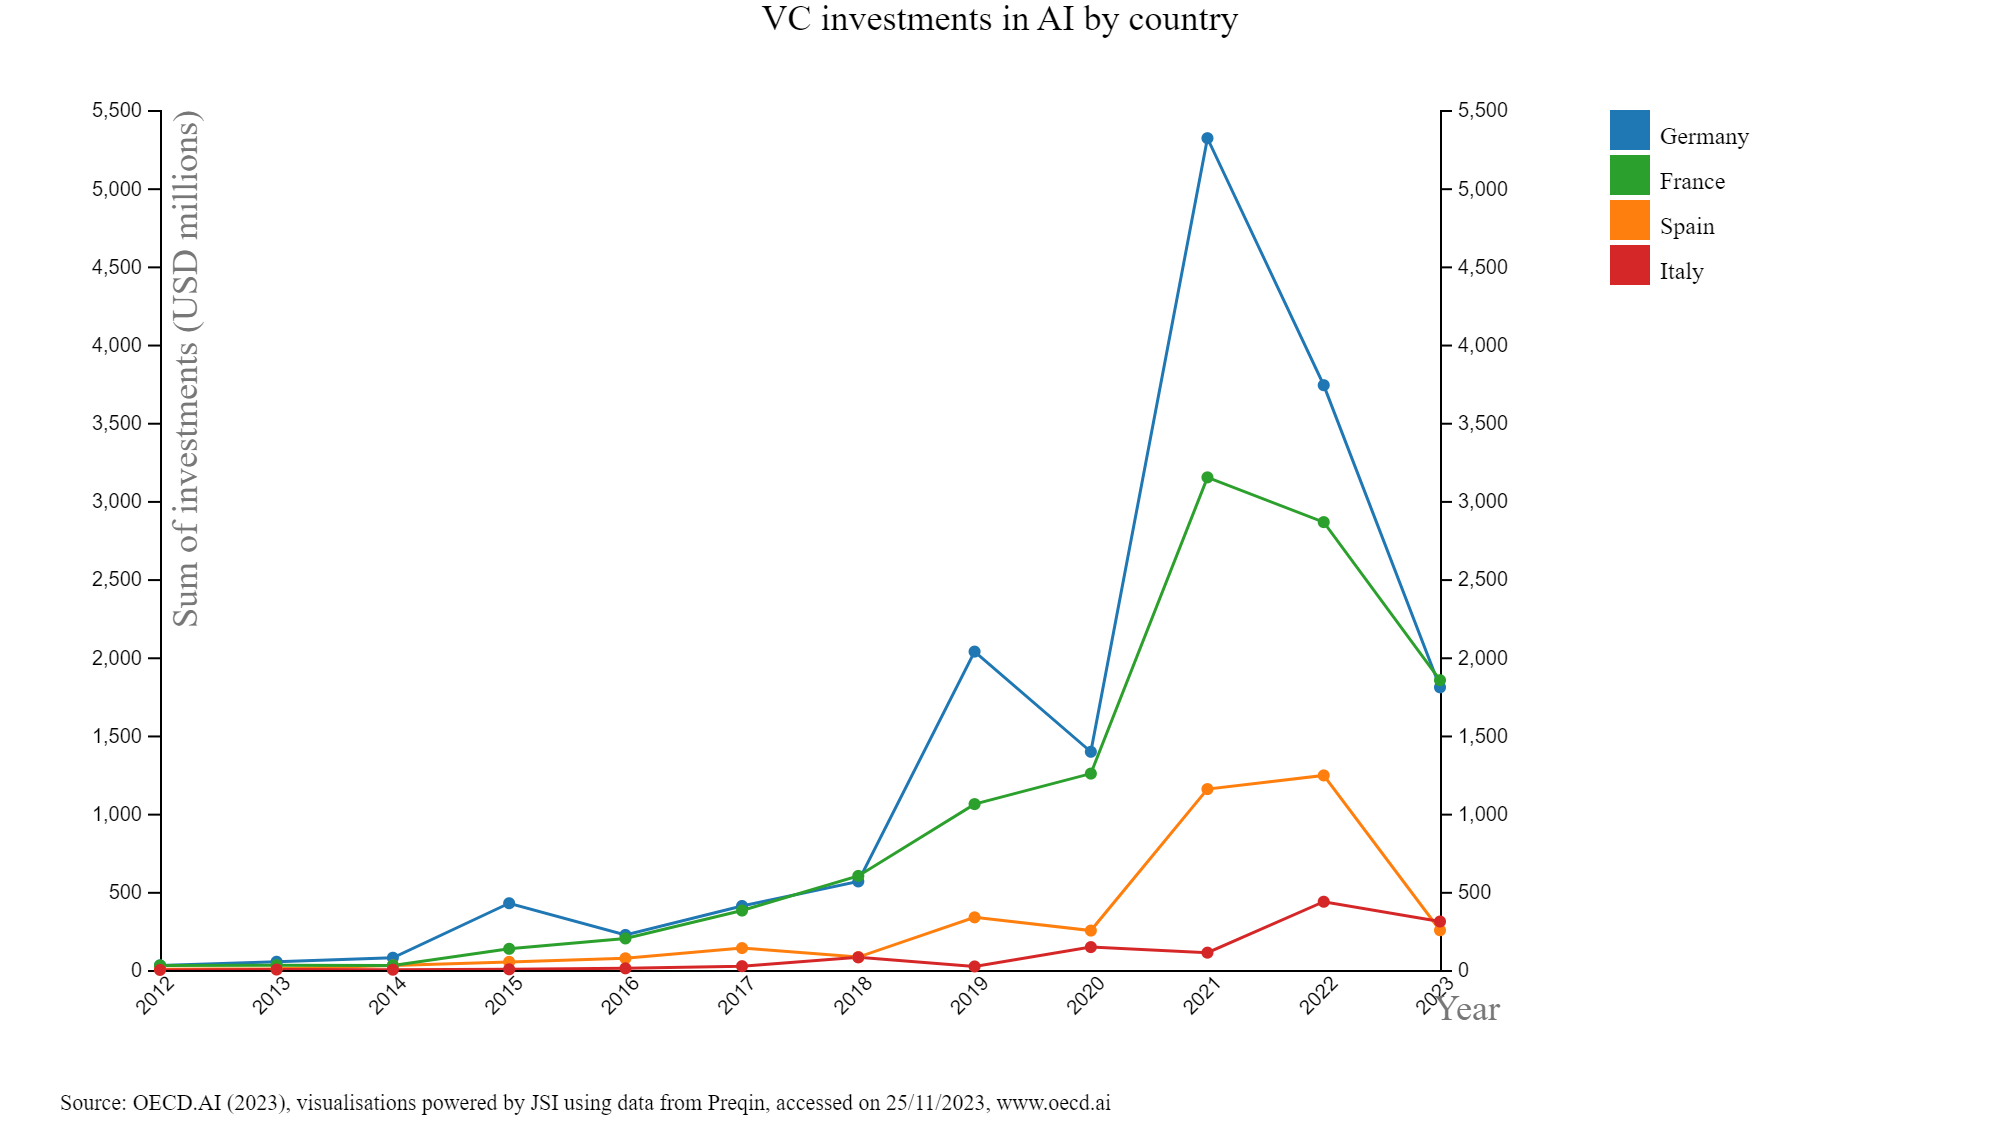
\includegraphics[width=0.3\linewidth]{Somma degli investimenti.png}
\end{center}   
Questo invece lo rappresenta sulla base dei milioni di dollari spesi in questo settore.\label{F:somma}
\begin{justify}
    
\end{justify}

\flushleft \subsection{Digitalizzazione dei contratti e principi}
Esempio.
\flushleft \subsection{Art 30 d.lgs 36/2023}
Esempio.
\flushleft \subsection{}
Esempio.

\newpage \centering
\section{Conclusione e opinioni finali}
\flushleft Esempio.

\end{document}
